\chapter{Signal systematics}\label{ch:signal_systematics}
There are several factors that contribute to the systematic uncertainty on the signal yields, which must be accounted for when checking for significant excesses in the signal region or when setting limits on signal production.
The size of the contribution from each source of uncertainty depends on the signal point being evaluated.
For each source of systematic uncertainty, a full set of signal Monte Carlo samples is generated with the value of a nuisance parameter shifted up, and another set is generated with the value of that parameter shifted down.
The spread in signal yields for each signal point between the two systematically-varied samples gives the size of that systematic uncertainty for that point.
For example, to evaluate the QCD scale uncertainty, two sets of signal samples are generated, one with the QCD scale shifted up by approximately 11\%, and one with the QCD scale shifted down by the same amount, and their signal yields are compared with the nominal signal yield.
Figures~\ref{fig:systematics_njet,fig:systematics_nbjet,fig:systematics_deta,fig:systematics_mj} shows the nominal and systematically-shifted distributions of four observables that contribute to the signal region definition for four representative signal points.
The nuisance parameters varied in these plots are the event internal weights of the PDF set, the QCD scale, and $\alpha_{S}$.

\begin{figure}[!ht]
    \centering
    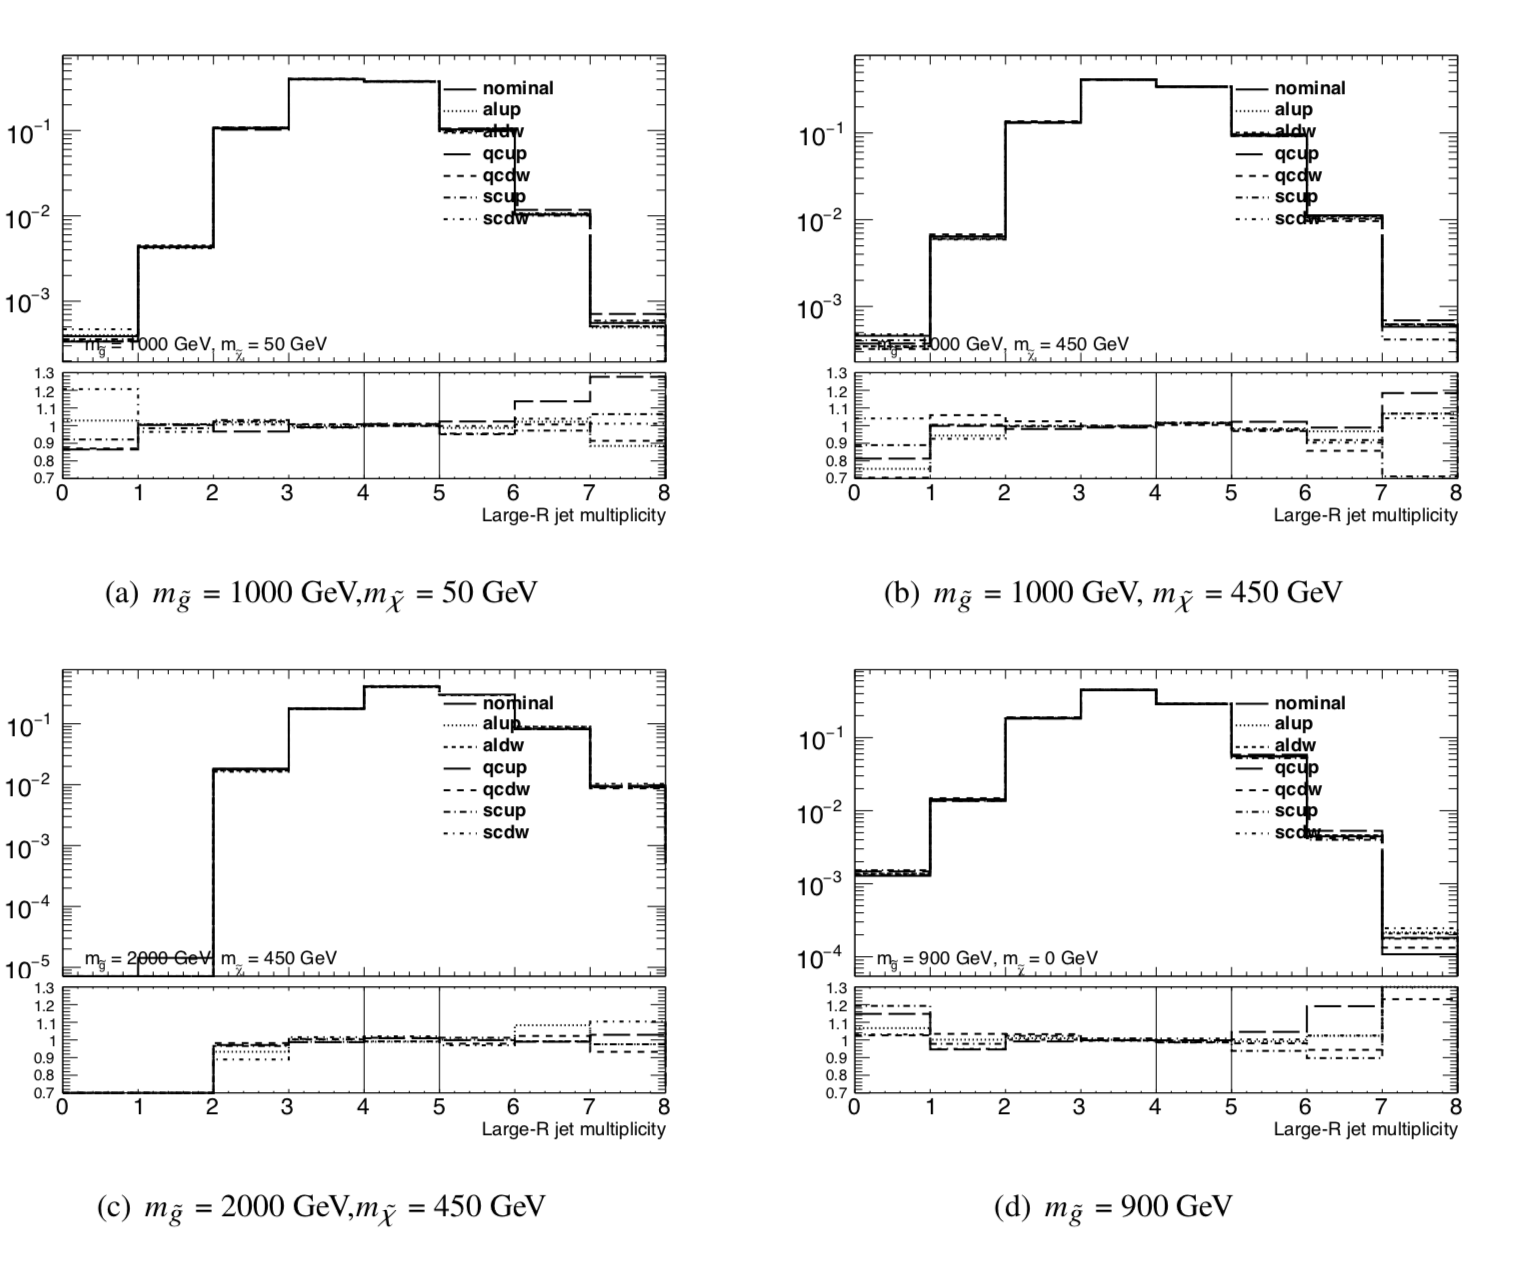
\includegraphics[width=0.9\textwidth]{systematics_njet_variation}
    \caption{Nominal and systematically-shifted $N_{jet}$ distributions for four signal points, showing the shifted distributions for internal generator event weights, QCD scale, and $\alpha_{s}$.}
    \label{fig:systematics_njet}
\end{figure}

\begin{figure}[!ht]
    \centering
    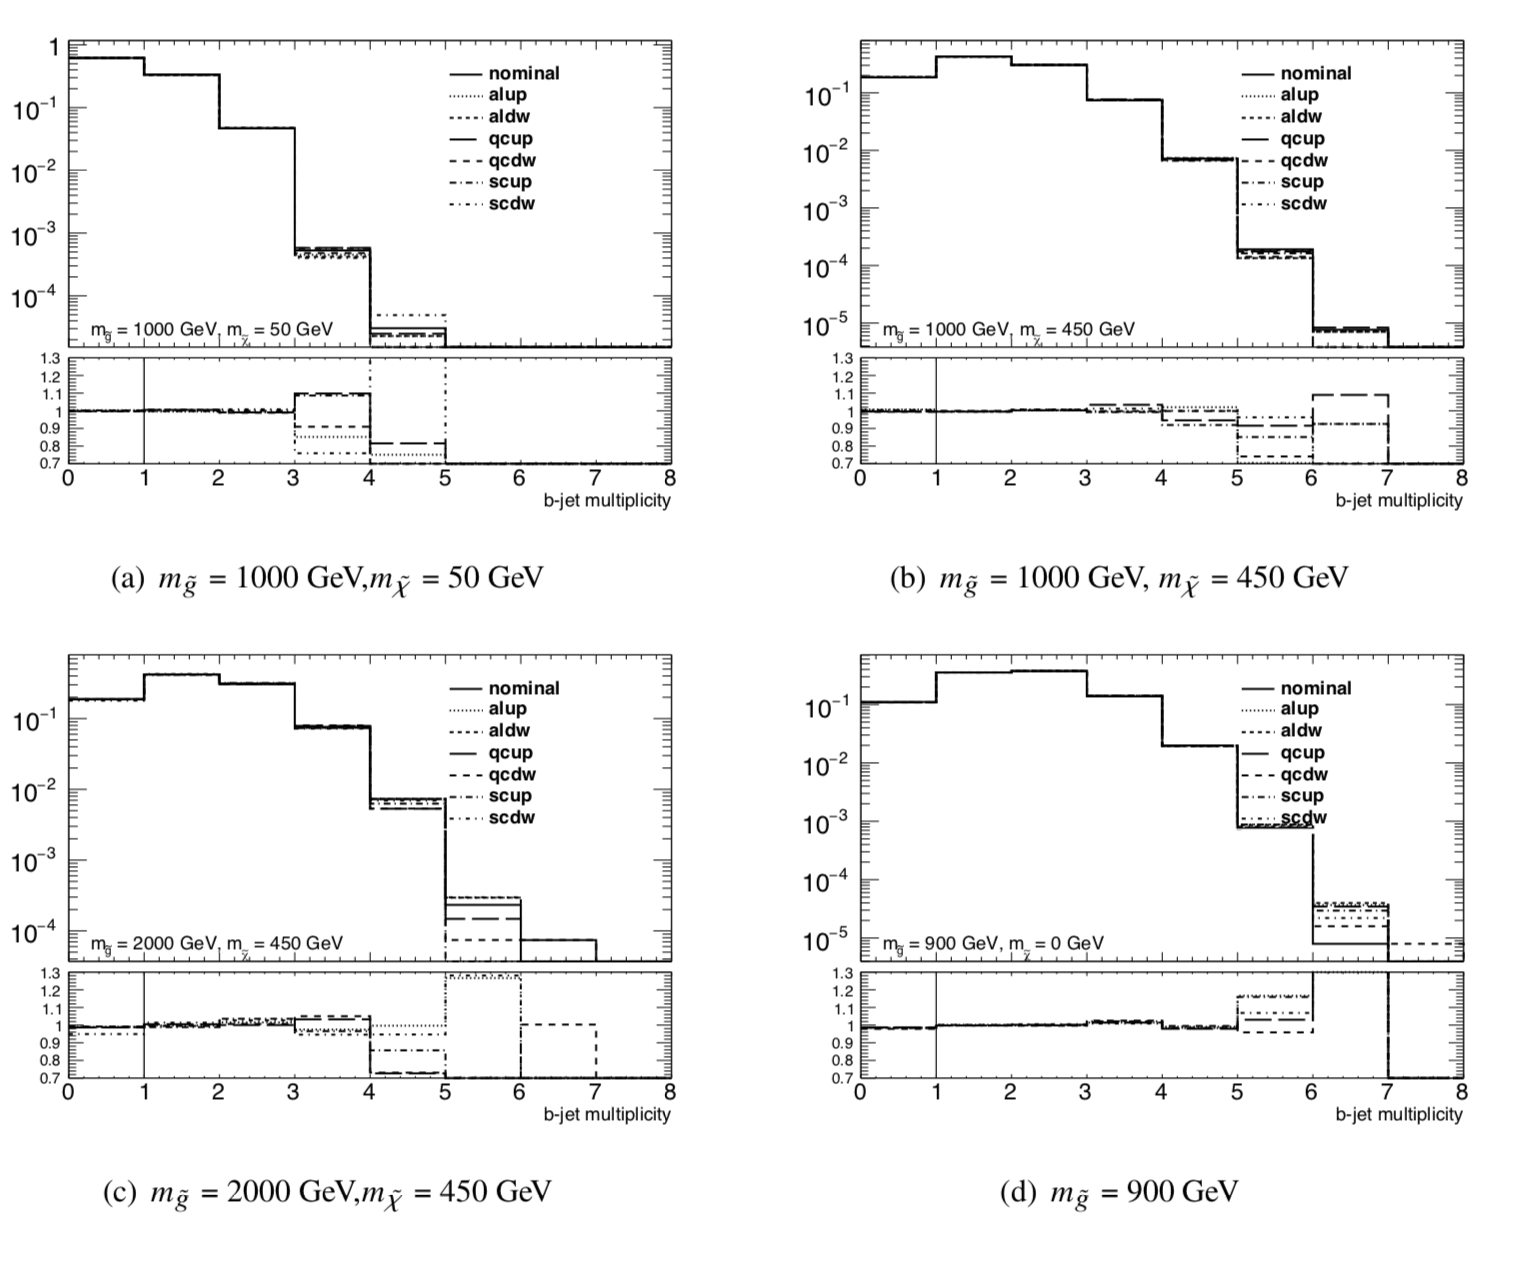
\includegraphics[width=0.9\textwidth]{systematics_nbjet_variation}
    \caption{Nominal and systematically-shifted $N_{b-jet}$ distributions for four signal points, showing the shifted distributions for internal generator event weights, QCD scale, and $\alpha_{s}$.}
    \label{fig:systematics_nbjet}
\end{figure}

\begin{figure}[!ht]
    \centering
    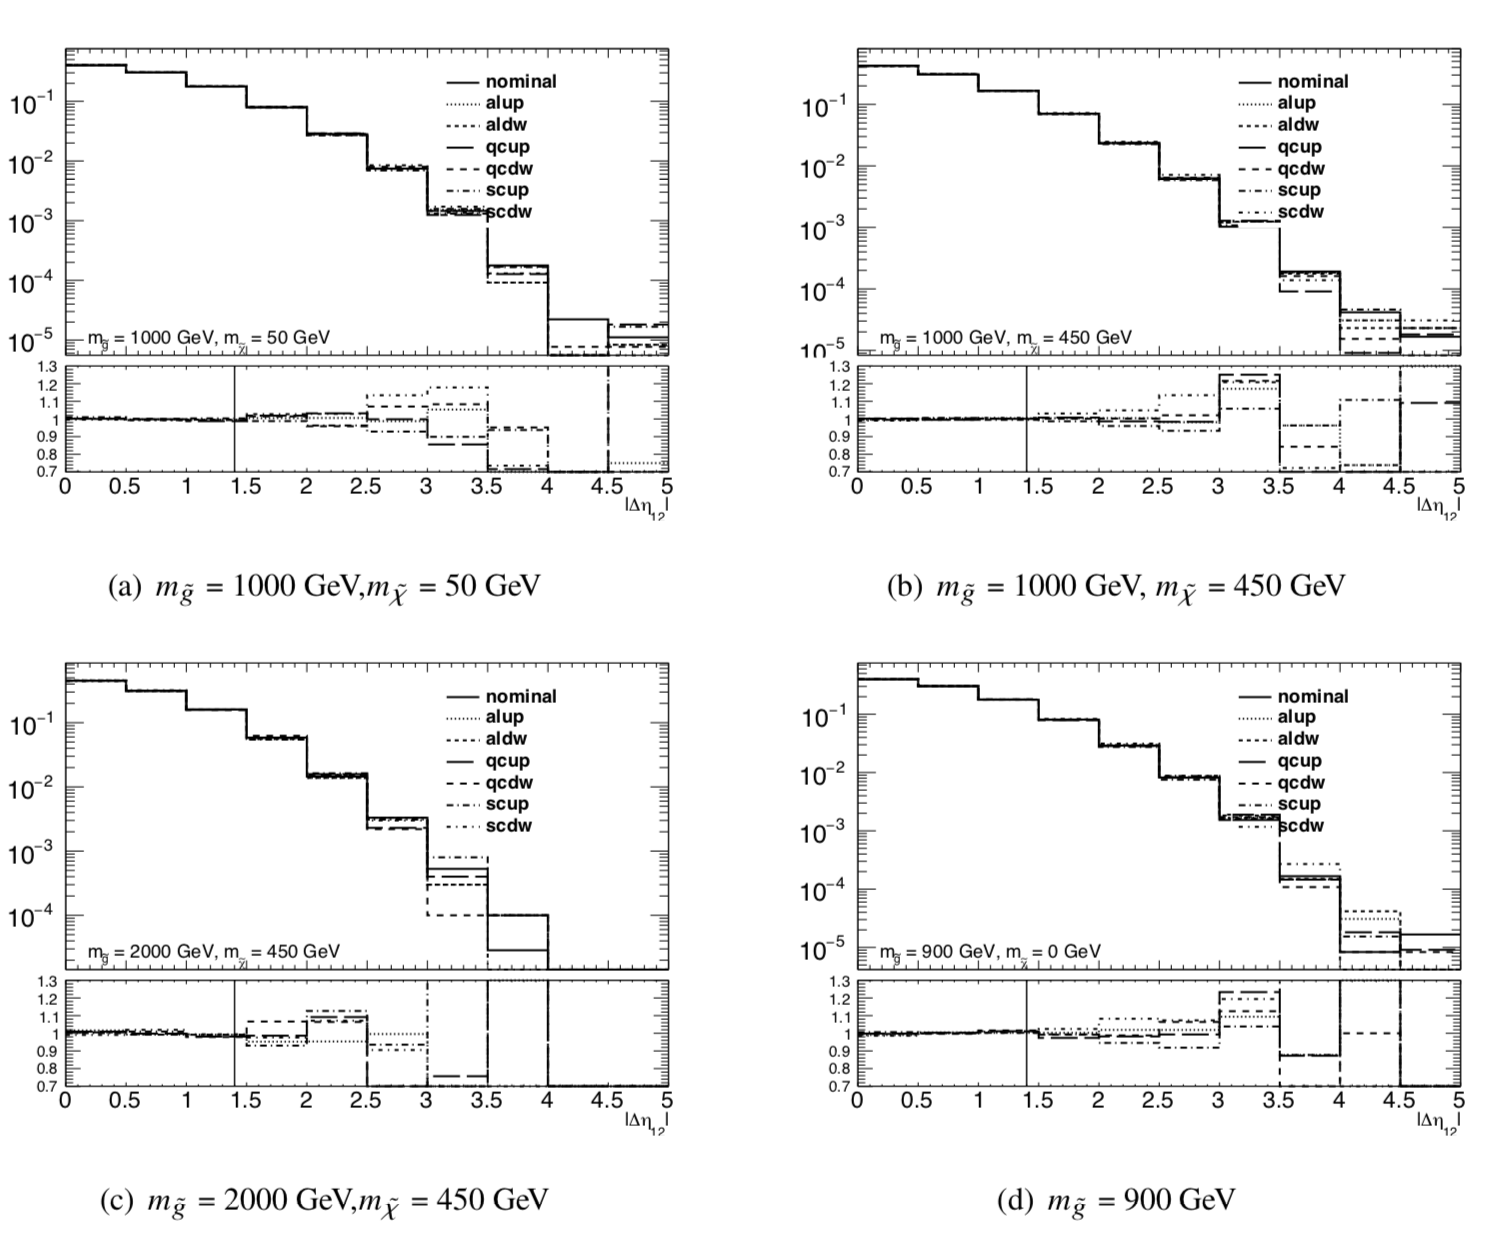
\includegraphics[width=0.9\textwidth]{systematics_deta_variation}
    \caption{Nominal and systematically-shifted $|\Delta\eta_{1,2}|$ distributions for four signal points, showing the shifted distributions for internal generator event weights, QCD scale, and $\alpha_{s}$.}
    \label{fig:systematics_deta}
\end{figure}

\begin{figure}[!ht]
    \centering
    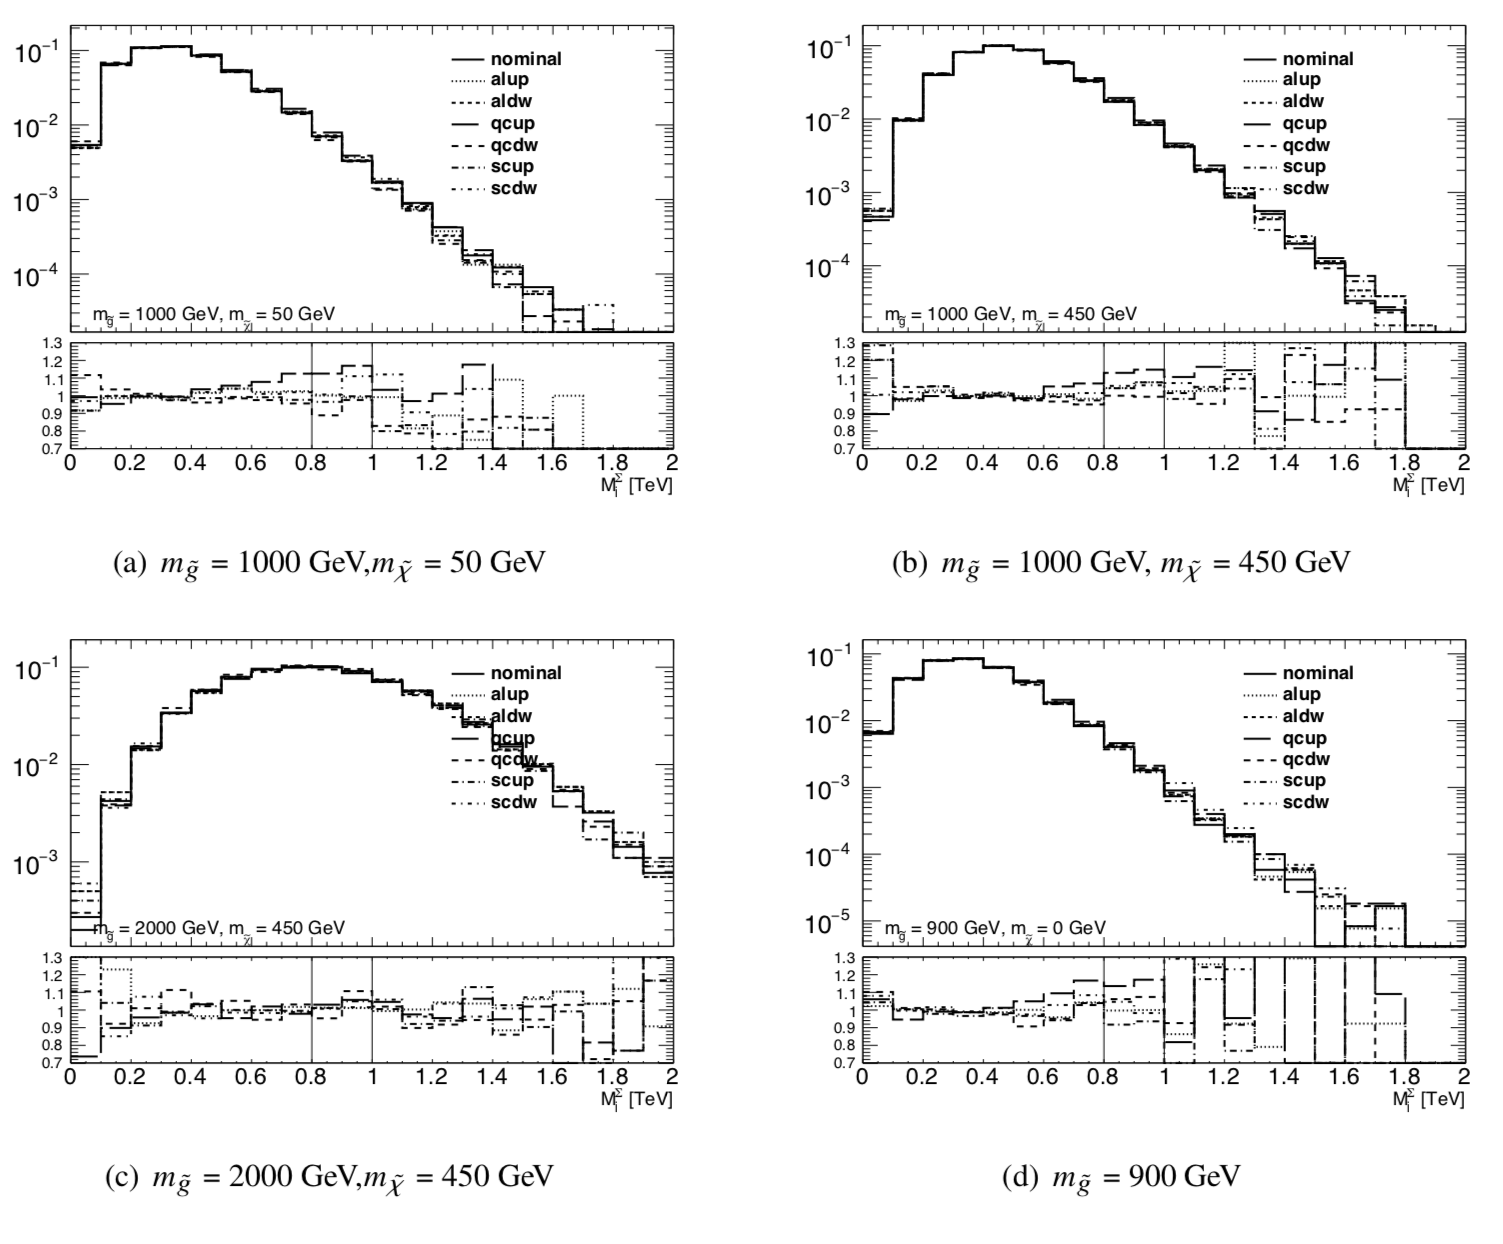
\includegraphics[width=0.9\textwidth]{systematics_mj_variation}
    \caption{Nominal and systematically-shifted $M_{J}^{\Sigma}$ distributions for four signal points, showing the shifted distributions for internal generator event weights, QCD scale, and $\alpha_{s}$.}
    \label{fig:systematics_mj}
\end{figure}


There are four main components to the systematic uncertainty on the estimated signal yield.
These components are the large-R jet mass scale (JMS), the small-R b-tagging uncertainty, the Monte Carlo statistical uncertainty, and the modelling uncertainty, which includes uncertainty on parton distribution functions (PDFs), QCD scale uncertainty, and initial state radiation (ISR) modelling uncertainty.
The size of a given systematic is evaluated by varying a nuisance parameter and determining the percent difference in signal yield between the nominal distribution and systematically varied distribution.
When a systematic contains multiple components, those components are treated as uncorrelated, and their contributions are combined in quadrature.
Systematic uncertainties depend on the gluino and neutralino masses being considered, as well as the decay mode of direct or cascade.
As such, they are evaluated separately at each point in the mass grid.

For the JMS uncertainty, there are four components, called the baseline, modeling, statistical, and tracking components.
These components are derived from the $R_{trk}$ method~\cite{jet-substructure-perf}.
The JMS uncertainty is largest for $m_{\tilde{g}}=1.0~TeV$, at $\approx 24\%$, and drops to $\approx 8\%$ for signal points with $m_{\tilde{g}}=1.8~TeV$.
It is generally dominated by the tracking uncertainty, followed by the baseline uncertainty.

The b-tagging uncertainty is evaluated by varying a set of 25 nuisance parameters.
The result is an uncertainty on the signal efficiency of between $15\%$ and $25\%$.
This uncertainty is only applied to the b-tag signal regions.

The Monte Carlo statistical uncertainty accounts for the fact that only a limited sample of simulated events are produced for each mass point.
The uncertainty is derived as $\sigma=\sqrt{\epsilon(1-\epsilon)/N}$, where $\epsilon$ is the efficiency measured in the sample, and $N$ is the sample size.

Evaluating the contribution to the signal efficiency uncertainty from PDF, $\alpha_s$ and ISR modelling uncertainties requires the generation of truth-level signal simulation samples where different parameters are varied in the generation.
For PDF uncertainties, the internal event weights in the PDF set are varied up and down during the generation.
For the QCD scale uncertainty, the value of $alpha_s$ is varied up and down during the generation.
For ISR uncertainties, the value of the matching scale, $q_{\textrm{cut}}$ is varied up and down during the generation.
The PDF and QCD scale contributions to the uncertainty are highest at low gluino mass, reaching a maximum of $25\%$ at$m_{\tilde{g}}=1.0~TeV$, the lowest gluino mass studied.
For higher masses, these uncertainties drop to only a few percent.
